% ============================================================
%  Projet Réussite - Dossier Technique
%  Auteur : Matthieu PELINGRE
%  M2SDD - Universite de Lorraine - 2025-2026
% ============================================================
\documentclass[12pt, a4paper, french]{report}

% ----------------------------------------------------------------
% Encodage et langue
% ----------------------------------------------------------------
\usepackage[utf8]{inputenc}
\usepackage[T1]{fontenc}
\usepackage[french]{babel}
\usepackage{lmodern}
\usepackage{microtype}

% ----------------------------------------------------------------
% Mise en page
% ----------------------------------------------------------------
\usepackage{geometry}
\geometry{
  top=2.5cm, bottom=2.5cm,
  left=2.8cm, right=2.8cm,
  headheight=15pt
}

% ----------------------------------------------------------------
% Couleurs (palette Python)
% ----------------------------------------------------------------
\usepackage{xcolor}
\definecolor{pythonblue}{HTML}{356D9C}
\definecolor{pythonyellow}{HTML}{FED03E}
\definecolor{pythondark}{HTML}{1E4068}
\definecolor{pythonlight}{HTML}{D6E8F5}
\definecolor{codeblue}{HTML}{3572A5}
\definecolor{codebg}{HTML}{F5F9FC}
\definecolor{codegreen}{HTML}{336633}
\definecolor{codegray}{HTML}{777777}

% ----------------------------------------------------------------
% En-tetes et pieds de page
% ----------------------------------------------------------------
\usepackage{fancyhdr}
\pagestyle{fancy}
\fancyhf{}
\fancyhead[L]{\small\color{pythonblue}\textit{Projet Réussite - Dossier Technique}}
\fancyhead[R]{\small\color{pythonblue}\textit{M2SDD 2025-2026}}
\fancyfoot[C]{\small\thepage}
\renewcommand{\headrulewidth}{0.4pt}

% ----------------------------------------------------------------
% Titres de chapitres et de sections
% ----------------------------------------------------------------
\usepackage{titlesec}
\titleformat{\chapter}[display]
  {\normalfont\huge\bfseries\color{pythondark}}
  {\color{pythonblue}\large\chaptertitlename\ \thechapter}
  {8pt}
  {\Huge\color{pythondark}}
  [\vspace{4pt}\color{pythonyellow}\rule{\textwidth}{2pt}]
\titlespacing*{\chapter}{0pt}{-10pt}{24pt}

\titleformat{\section}{\large\bfseries\color{pythonblue}}{\thesection}{1em}{}
\titleformat{\subsection}{\normalsize\bfseries\color{pythondark}}{\thesubsection}{1em}{}
\titleformat{\subsubsection}{\normalsize\itshape\color{pythonblue}}{\thesubsubsection}{1em}{}

% ----------------------------------------------------------------
% Graphiques, figures, tableaux
% ----------------------------------------------------------------
\usepackage{graphicx}
\usepackage{float}
\usepackage{caption}
\usepackage{subcaption}
\usepackage{booktabs}
\usepackage{array}
\captionsetup{font=small, labelfont={bf,color=pythonblue}}

% ----------------------------------------------------------------
% TikZ (conserve pour usage futur, figures externalisees)
% ----------------------------------------------------------------
\usepackage{tikz}
\usetikzlibrary{positioning, arrows.meta, fit, backgrounds}

% ----------------------------------------------------------------
% Listings (code Python)
% ----------------------------------------------------------------
\usepackage{listings}
\lstdefinestyle{python}{
  language=Python,
  basicstyle=\small\ttfamily,
  keywordstyle=\color{codeblue}\bfseries,
  stringstyle=\color{codegreen},
  commentstyle=\color{codegray}\itshape,
  numberstyle=\tiny\color{codegray},
  numbers=left, stepnumber=1, numbersep=6pt,
  breaklines=true, breakatwhitespace=false,
  frame=single, rulecolor=\color{pythonblue!30},
  backgroundcolor=\color{codebg},
  tabsize=4, showstringspaces=false,
  captionpos=b,
  morekeywords={Optional, Union, Dict, Tuple, List, Any, ABC, abstractmethod}
}
\lstdefinestyle{bash}{
  language=bash,
  basicstyle=\small\ttfamily,
  keywordstyle=\color{codeblue},
  commentstyle=\color{codegray}\itshape,
  numbers=none,
  frame=single, rulecolor=\color{pythonblue!30},
  backgroundcolor=\color{codebg},
  breaklines=true,
  captionpos=b
}
\lstset{style=python}

% ----------------------------------------------------------------
% Boites colorees (tcolorbox)
% ----------------------------------------------------------------
\usepackage{tcolorbox}
\tcbuselibrary{skins, breakable}

\newtcolorbox{patternbox}[1]{
  colback=pythonyellow!15, colframe=pythonyellow!60!pythonblue,
  coltitle=pythondark, fonttitle=\bfseries,
  title={#1}, arc=4pt, boxrule=1pt
}

\newtcolorbox{notebox}{
  colback=pythonlight, colframe=pythonblue,
  fonttitle=\bfseries, title={Remarque},
  arc=4pt, boxrule=1pt
}

% ----------------------------------------------------------------
% Liens
% ----------------------------------------------------------------
\usepackage{hyperref}
\hypersetup{
  colorlinks=true,
  linkcolor=pythondark,
  urlcolor=pythonblue,
  citecolor=pythondark,
  pdftitle={Projet Réussite - Dossier Technique},
  pdfauthor={Matthieu PELINGRE}
}

% ----------------------------------------------------------------
% Listes et maths
% ----------------------------------------------------------------
\usepackage{enumitem}
\setlist[itemize]{leftmargin=*, itemsep=2pt}
\setlist[enumerate]{leftmargin=*, itemsep=2pt}
\usepackage{amsmath}

% ============================================================
%  DOCUMENT
% ============================================================
\begin{document}

% ----------------------------------------------------------------
% Page de garde
% ----------------------------------------------------------------
\begin{titlepage}
  \centering
  \vspace*{1.5cm}

  {\large\color{pythonblue} Université de Lorraine - Master 2 Sciences des Données (M2SDD)}\\[0.4cm]
  {\normalsize Projet commun : Algorithmique \textperiodcentered{}
    Programmation \textperiodcentered{}
    Mathématiques pour l'informatique}\\[0.3cm]
  {\normalsize Année universitaire 2025-2026}

  \vspace{1.5cm}
  \noindent\rule{\textwidth}{2pt}\\[0.3cm]
  {\Huge\bfseries\color{pythondark} Projet Réussite}\\[0.5cm]
  {\LARGE\color{pythonblue} Dossier Technique}\\[0.3cm]
  \noindent\rule{\textwidth}{2pt}

  \vspace{1.5cm}

  \begin{tcolorbox}[colback=pythonlight, colframe=pythonblue, arc=6pt, boxrule=1.5pt]
    \centering
    \textit{Prédiction de la réussite d'un apprenant\\
    à partir de ses traces numériques sur la plateforme ARCHE}
  \end{tcolorbox}

  \vspace{2cm}

  \begin{tabular}{ll}
    \textbf{Auteur :}  & Matthieu PELINGRE \\
    \textbf{Email :}   & matthieu.pelingre1@etu.univ-lorraine.fr \\
    \textbf{Dépôt :} & \href{https://github.com/M2SDD/projet-reussite}{github.com/M2SDD/projet-reussite} \\
    \textbf{Date :}    & Avril 2026 \\
  \end{tabular}

  \vfill

  {\small\color{gray}
    Logiciel développé en Python~3 \textperiodcentered{}
    Tkinter \textperiodcentered{} scikit-learn \textperiodcentered{}
    pandas \textperiodcentered{} matplotlib
  }
\end{titlepage}

% ----------------------------------------------------------------
% Table des matieres
% ----------------------------------------------------------------
\tableofcontents
\clearpage

% ============================================================
\chapter{Architecture générale du logiciel}
% ============================================================

\section{Vue d'ensemble}

Le logiciel \textbf{Projet Réussite} est une application orientée objet de bureau développée en Python~3.
L'application réalise un pipeline complet allant du chargement des données brutes jusqu'à la comparaison de modèles de prédiction, avec une interface graphique \texttt{Tkinter}.

L'ensemble du code source est organisé dans le répertoire \texttt{src/}, structuré en sous-paquets thématiques. Le point d'entrée unique est \texttt{main.py}, à la racine du projet.

\subsection{Structure des répertoires}

\begin{lstlisting}[style=bash, caption={Arborescence du projet}]
projet_reussite/
|-- main.py                       # Point d'entree
|-- data/
|   |-- logs_info_25_pseudo.csv
|   `-- notes_info_25_pseudo.csv
`-- src/
    |-- config.py                 # Configuration centralisee
    |-- data/
    |   |-- data_loader.py        # Chargement et validation
    |   |                         # CSV
    |   |-- feature_extractor.py  # Feature Engineering
    |   |-- data_cleaner.py       # Nettoyage et selection de
    |   |                         # variables
    |   |-- dataset_builder.py    # Orchestrateur ETL
    |   `-- statistics_module.py  # Statistiques descriptives
    |-- models/
    |   |-- base_regressor.py     # Classe abstraite de base
    |   |-- linear_regressor.py
    |   `-- ensemble_regressor.py
    |-- evaluation/
    |   `-- model_evaluator.py
    |-- visualization/
    |   `-- model_visualizer.py
    `-- interface/
        |-- app_controller.py     # Controleur MVC
        |-- main_window.py        # Fenetre principale
        |-- tabs/                 # Quatre onglets (Vues MVC)
        `-- widgets/              # Composants reutilisables
\end{lstlisting}

\section{Architecture Modèle-Vue-Contrôleur (MVC)}

L'application suit une architecture \textbf{Modèle-Vue-Contrôleur} (MVC). Ce choix architectural répond à la contrainte d'une interface graphique \texttt{Tkinter} tout en séparant clairement la logique métier de la présentation.

\resizebox{0.9\textwidth}{!}{
\begin{tikzpicture}[
  layerlabel/.style={font=\bfseries\small\color{pythondark}, align=center},
  classnode/.style={
    draw=pythonblue, fill=white, thick,
    minimum width=3.8cm, minimum height=0.75cm,
    font=\small\ttfamily, align=center,
    rounded corners=2pt
  },
  arrow/.style={-{Stealth[length=6pt]}, thick, pythonblue!70},
  groupbox/.style={draw=pythonblue!50, thick, dashed, rounded corners=6pt,
                   inner sep=10pt, fill=pythonlight!40}
]

% ---- COUCHE MODELE ----
\begin{scope}
  \node[classnode, fill=pythonlight] (cfg)  at (0, 9.0)  {\textbf{Config}};
  \node[classnode]                   (dl)   at (0, 8.0)  {DataLoader};
  \node[classnode]                   (fe)   at (0, 7.0)  {FeatureExtractor};
  \node[classnode]                   (dc)   at (0, 6.0)  {DataCleaner};
  \node[classnode]                   (db)   at (0, 5.0)  {DatasetBuilder};
  \node[classnode]                   (sm)   at (0, 4.0)  {StatisticsModule};
  \node[classnode, draw=pythonblue!70, dashed,
        font=\small\ttfamily\itshape] (br)  at (0, 3.0)  {BaseRegressor};
  \node[classnode]                   (lr)   at (-2.1, 2.0) {LinearRegressor};
  \node[classnode]                   (er)   at ( 2.1, 2.0) {EnsembleRegressor};
  \node[classnode]                   (me)   at (0, 1.0)  {ModelEvaluator};
  \node[classnode]                   (mv)   at (0, 0.0)  {ModelVisualizer};

  \begin{scope}[on background layer]
    \node[groupbox, fit=(cfg)(dl)(fe)(dc)(db)(sm)(br)(lr)(er)(me)(mv)] (modelbox) {};
  \end{scope}
  \node[layerlabel, above=2pt of modelbox.north] {MODÈLE};
\end{scope}

% ---- COUCHE CONTROLEUR ----
\begin{scope}
  \node[classnode, fill=pythonyellow!30, draw=pythonyellow!60!pythondark,
        minimum width=4cm, minimum height=1.2cm,
        font=\normalsize\bfseries\ttfamily]
    (ac) at (9, 4.5) {AppController};

  \begin{scope}[on background layer]
    \node[groupbox, fill=pythonyellow!10, draw=pythonyellow!60!pythondark,
          fit=(ac), inner sep=18pt] (ctrlbox) {};
  \end{scope}
  \node[layerlabel, above=2pt of ctrlbox.north] {CONTRÔLEUR};
\end{scope}

% ---- COUCHE VUE ----
\begin{scope}
  \node[classnode, fill=green!15, draw=green!50!black]
    (mw)  at (16, 7.5) {MainWindow};
  \node[classnode] (t1)  at (16, 6.5) {DataTab};
  \node[classnode] (t2)  at (16, 5.5) {PreprocessingTab};
  \node[classnode] (t3)  at (16, 4.5) {ModelingTab};
  \node[classnode] (t4)  at (16, 3.5) {EvaluationTab};
  \node[classnode] (sb)  at (16, 2.5) {StatusBar};
  \node[classnode] (dfv) at (16, 1.5) {DataFrameViewer};

  \begin{scope}[on background layer]
    \node[groupbox, fill=green!5, draw=green!50!black,
          fit=(mw)(t1)(t2)(t3)(t4)(sb)(dfv)] (viewbox) {};
  \end{scope}
  \node[layerlabel, above=2pt of viewbox.north] {VUE};
\end{scope}

% ---- Flèches entre couches ----
\draw[arrow, <->] (modelbox.east) -- (ctrlbox.west)
  node[midway, above, font=\tiny\itshape, color=pythonblue]{utilise};

\draw[arrow, <->] (ctrlbox.east) -- (viewbox.west)
  node[midway, above, font=\tiny\itshape, color=pythonblue]{notifie};

\end{tikzpicture}
}

\begin{description}[leftmargin=2.5cm, style=nextline]
  \item[\textbf{Modèle}]
    Regroupe toutes les classes métier : chargement des données (\texttt{DataLoader}),
    extraction de variables (\texttt{FeatureExtractor}), nettoyage (\texttt{DataCleaner}),
    orchestration (\texttt{DatasetBuilder}), modèles prédictifs (\texttt{BaseRegressor}
    et ses sous-classes) et évaluation (\texttt{ModelEvaluator}).
    Ces classes sont indépendantes de l'interface graphique.

  \item[\textbf{Contrôleur}]
    La classe \texttt{AppController} constitue l'unique point de communication entre
    la vue et le modèle. Elle maintient l'état global de l'application
    (données chargées, dataset construit, modèles entraînés) et expose des méthodes
    métier de haut niveau. Les onglets ne font \emph{jamais} d'appels directs aux
    classes du modèle.

  \item[\textbf{Vue}]
    \texttt{MainWindow} crée le \texttt{ttk.Notebook} et les quatre onglets.
    Chaque onglet est une classe autonome gérant ses propres widgets Tkinter.
    La vue ne contient aucune logique métier.
\end{description}

\section{Patrons de conception utilisés}

Trois patrons de conception (\textit{design patterns}) structurent l'application.

\begin{patternbox}{Patron 1 : \texttt{BaseRegressor} (Template Method)}
La classe abstraite \texttt{BaseRegressor} définit le squelette de l'algorithme d'entraînement dans sa méthode publique \texttt{fit()} : validation des données, mise à l'échelle, puis appel à \texttt{\_fit()}. La méthode \texttt{\_fit()} est abstraite et doit être implémentée par chaque sous-classe (\texttt{LinearRegressor}, \texttt{EnsembleRegressor}).
Cela garantit que toutes les validations et le scaling sont toujours effectués, quelle que soit l'implémentation concrète.
\end{patternbox}

\begin{patternbox}{Patron 2 : \texttt{DatasetBuilder} (Facade Pattern)}
\texttt{DatasetBuilder} orchestre trois composants (\texttt{DataLoader}, \texttt{FeatureExtractor}, \texttt{DataCleaner}) en exposant une interface unifiée via la méthode \texttt{build\_dataset()}. Le contrôleur n'a pas besoin de connaître les détails de chaque étape du pipeline.
\end{patternbox}

\begin{patternbox}{Patron 3 : \texttt{DataCleaner.select\_features()} (Strategy Pattern)}
La méthode \texttt{select\_features()} de \texttt{DataCleaner} accepte une liste de méthodes de sélection (\texttt{'linear'}, \texttt{'mutual\_info'}, \texttt{'importance'}, \texttt{'rfe'}) et délègue à la méthode correspondante.
Cette approche permet de combiner plusieurs stratégies de sélection sans modifier le code appelant.
\end{patternbox}

% ============================================================
\chapter{Diagramme de classes}
% ============================================================

\section{Hiérarchie des modèles de prédiction}

\begin{figure}[H]
  \centering
  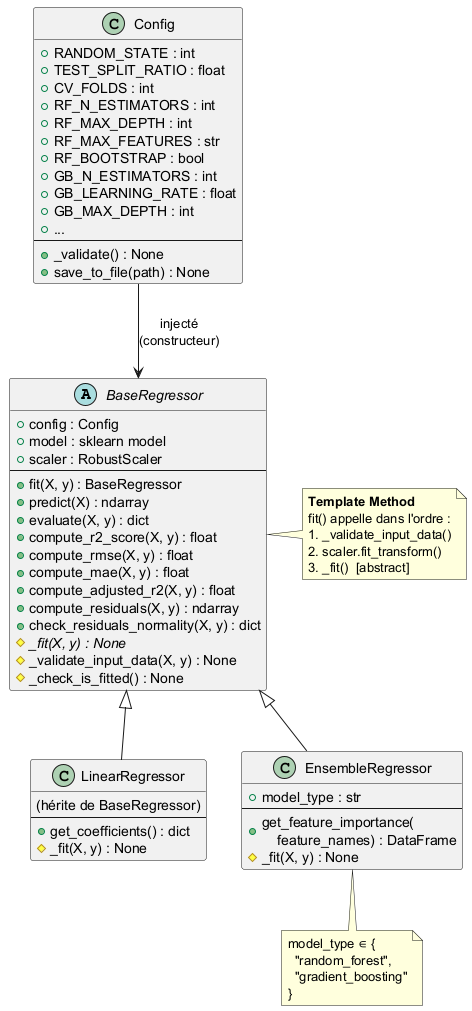
\includegraphics[width=0.5\textwidth]{figures/fig_hierarchy.png}
  \caption{Hiérarchie d'héritage des classes de modèles de prédiction}
\end{figure}

La relation d'héritage entre \texttt{BaseRegressor} et ses sous-classes illustre le patron \textit{Template Method} : la logique commune (scaling, validation, calcul des métriques) est centralisée dans la classe abstraite, tandis que chaque sous-classe n'implémente que la logique qui lui est propre via la méthode \texttt{\_fit()}.

\section{Pipeline de préparation des données}

\resizebox{\textwidth}{!}{
\begin{tikzpicture}[
  component/.style={
    draw=pythonblue, fill=white, thick,
    minimum width=3.5cm, minimum height=2.2cm,
    align=center, font=\small, rounded corners=3pt,
    inner sep=8pt
  },
  io/.style={
    draw=gray!60, fill=gray!10, thick,
    minimum width=2.5cm, minimum height=1.4cm,
    align=center, font=\small, rounded corners=3pt
  },
  arrow/.style={-{Stealth[length=8pt, width=5pt]}, very thick, gray!70},
  ioarrow/.style={-{Stealth[length=8pt, width=5pt]}, thick, gray!70},
  label/.style={font=\tiny\itshape, color=pythonblue, align=center}
]

% ---- Entrée ----
\node[io] (csv) at (-5.5, 0) {
  \textbf{Fichiers CSV}\\[3pt]
  \texttt{logs.csv}\\
  \texttt{notes.csv}
};

% ---- DataLoader ----
\node[component, fill=pythonlight!60] (dl) at (0, 0) {
  \textbf{DataLoader}\\[4pt]
  \texttt{load\_logs()}\\
  \texttt{load\_notes()}\\[4pt]
  \tiny Validation colonnes\\
  \tiny Parsing datetime
};

% ---- FeatureExtractor ----
\node[component, fill=pythonlight!60] (fe) at (5.5, 0) {
  \textbf{FeatureExtractor}\\[4pt]
  \texttt{extract\_features()}\\[4pt]
  \tiny Métriques d'activité\\
  \tiny Patterns temporels\\
  \tiny Composants ARCHE\\
  \tiny Régularité
};

% ---- DataCleaner ----
\node[component, fill=pythonlight!60] (dc) at (11, 0) {
  \textbf{DataCleaner}\\[4pt]
  \texttt{remove\_duplicates()}\\
  \texttt{select\_features()}\\[4pt]
  \tiny Filtre variance\\
  \tiny Filtre corrélation\\
  \tiny SelectKBest / RFE
};

% ---- Sortie ----
\node[io] (out) at (16.5, 0) {
  \textbf{Dataset}\\[3pt]
  \texttt{X} (features)\\
  \texttt{y} (notes)
};

% Flèches entre composants
\draw[ioarrow] (csv.east) -- (dl.west)
  node[midway, above, label]{df\_logs\\df\_notes};

\draw[arrow] (dl.east) -- (fe.west)
  node[midway, above, label]{df\_logs};

\draw[arrow] (fe.east) -- (dc.west)
  node[midway, above, label]{df\_features\\(1 ligne/étudiant)};

\draw[ioarrow] (dc.east) -- (out.west)
  node[midway, above, label]{k variables\\sélectionnées};

% Jointure notes (flèche depuis DataLoader vers DataCleaner via le bas)
\draw[arrow, gray!50, dashed] (dl.south) -- ++(0, -1.0)
  -- node[below, label, color=gray]{Jointure notes (inner join)} ++(11, 0)
  -- (dc.south);

% ---- Boîte DatasetBuilder (façade) ----
\begin{scope}[on background layer]
  \node[
    draw=pythondark, dashed, thick,
    fill=pythonyellow!8,
    rounded corners=8pt,
    fit=(dl)(fe)(dc),
    inner sep=14pt,
    label={[font=\bfseries\small\color=pythondark]above:DatasetBuilder \textit{(Façade)}}
  ] (dsb) {};
\end{scope}

\end{tikzpicture}
}

Le \texttt{DatasetBuilder} encapsule les trois composants du pipeline de données. Le contrôleur (\texttt{AppController}) invoque uniquement \texttt{build\_dataset()} et reçoit directement les matrices \texttt{X} et \texttt{y} prêtes à l'emploi.

\section{Module d'évaluation}

\begin{figure}[H]
  \centering
  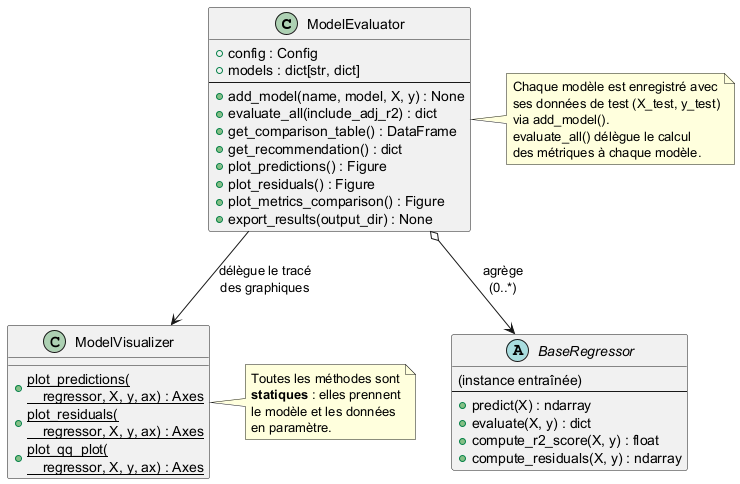
\includegraphics[width=0.85\textwidth]{figures/fig_evaluator.png}
  \caption{Classes du module d'évaluation et leurs relations}
\end{figure}

\texttt{ModelEvaluator} centralise la comparaison des modèles enregistrés et délègue la génération des graphiques à \texttt{ModelVisualizer}, dont toutes les méthodes sont statiques.

% ============================================================
\chapter{Conception de l'interface utilisateur}
% ============================================================

\section{Principes de conception}

L'interface graphique est construite avec \textbf{Tkinter/ttk} (bibliothèque standard Python). Elle est organisée autour d'un \texttt{ttk.Notebook} à quatre onglets, activés progressivement au fil du pipeline. 
Ce mécanisme d'activation progressive guide l'utilisateur et prévient toute erreur d'utilisation.

\begin{center}
\begin{tabular}{clll}
\toprule
\textbf{N°} & \textbf{Onglet} & \textbf{Condition d'activation} & \textbf{Classe}\\
\midrule
0 & Données         & Toujours actif                    & \texttt{DataTab}\\
1 & Prétraitement   & Après chargement des CSV          & \texttt{PreprocessingTab}\\
2 & Modélisation    & Après construction du dataset     & \texttt{ModelingTab}\\
3 & Évaluation      & Après entraînement d'un modèle    & \texttt{EvaluationTab}\\
\bottomrule
\end{tabular}
\end{center}


\section{Onglet 1 : Données}

\begin{figure}[H]
  \centering
  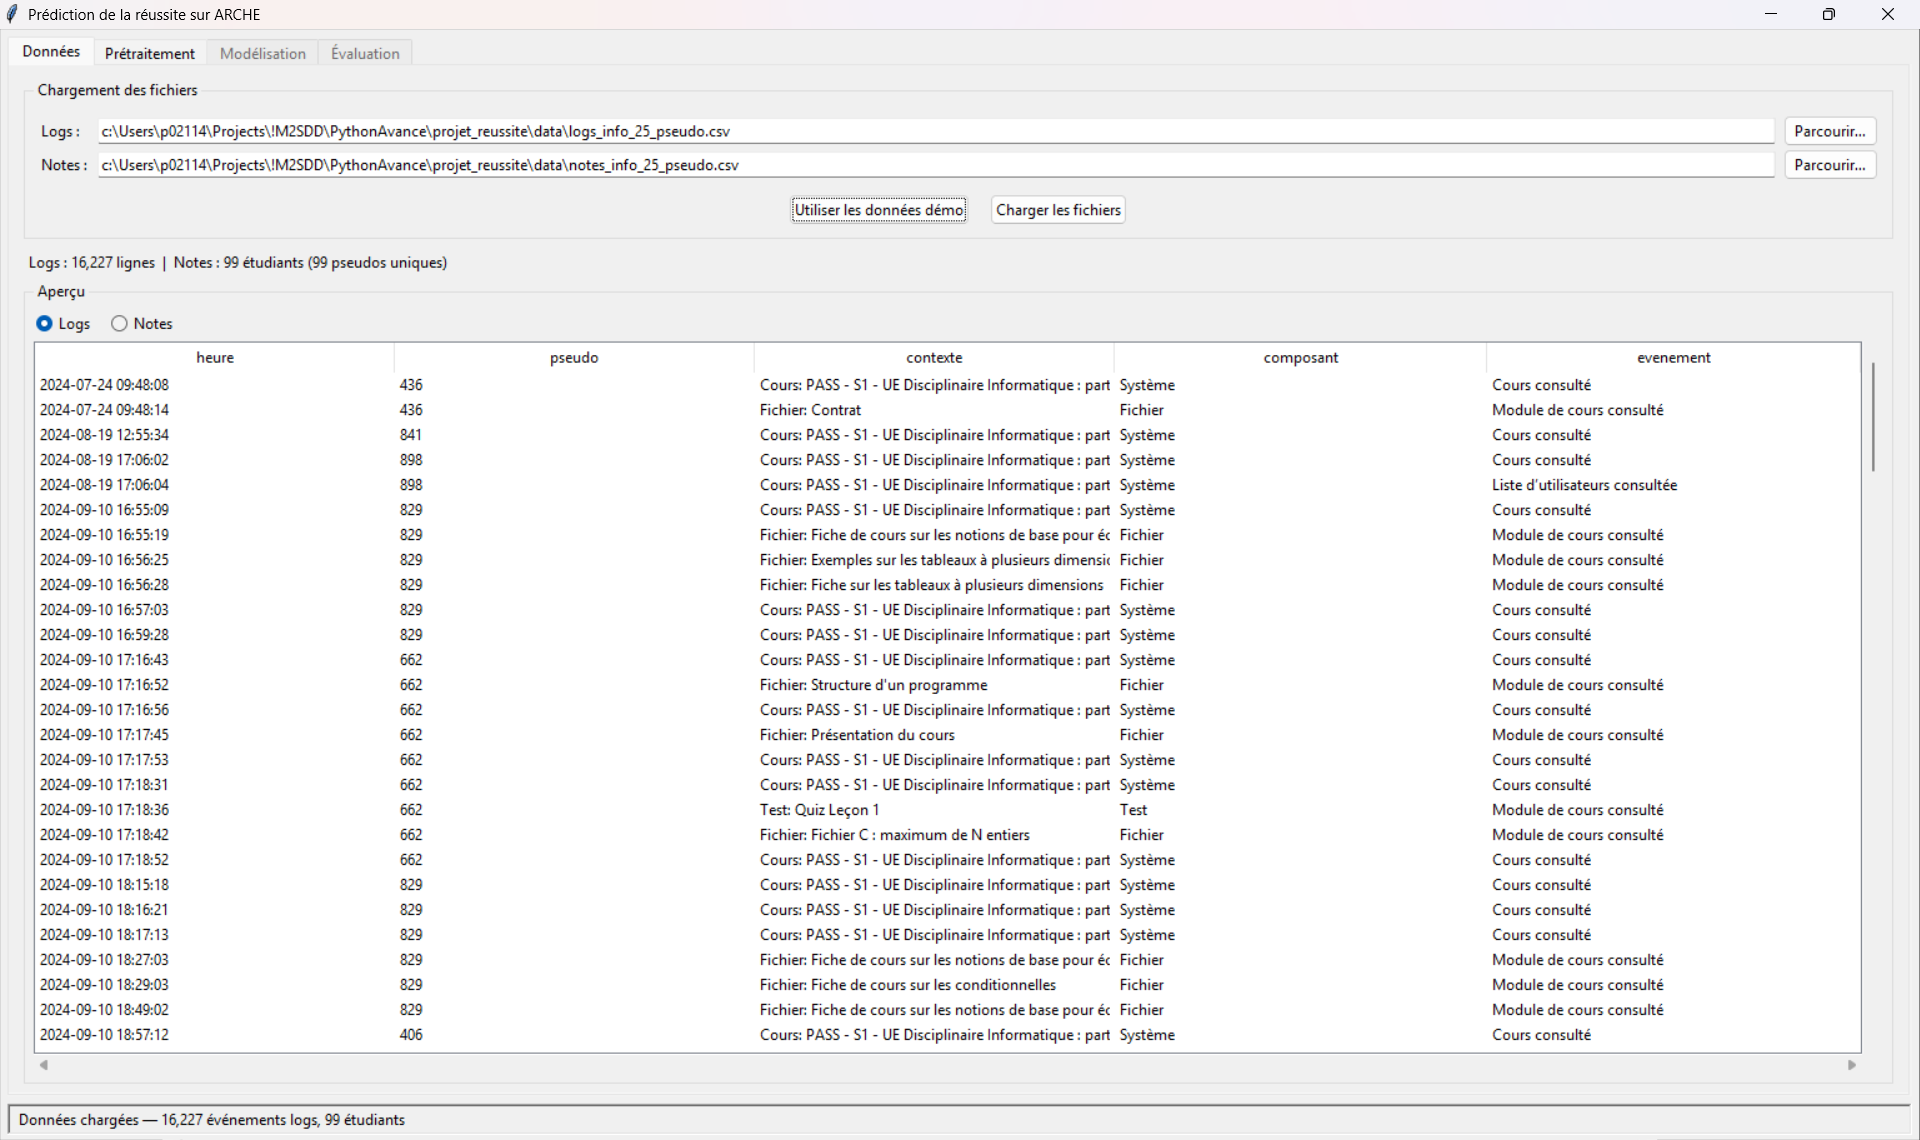
\includegraphics[width=0.92\textwidth]{../pictures/onglet1.png}
  \caption{Onglet \textit{Données} : Chargement et aperçu des fichiers CSV}
\end{figure}


\noindent L'onglet \textbf{Données} permet à l'utilisateur de :
\begin{itemize}
  \item sélectionner les deux fichiers CSV (logs et notes) via un dialogue système, ou charger directement les fichiers de démonstration inclus.
  \item visualiser un aperçu tabulaire (\texttt{DataFrameViewer}) de chaque fichier, basculé par boutons radio (Logs / Notes).
  \item consulter un résumé (nombre de lignes, d'étudiants, de pseudos uniques).
\end{itemize}

Le chargement s'effectue dans un \textbf{thread secondaire} (module \texttt{threading}) pour éviter de bloquer l'interface lors du traitement de fichiers volumineux.

\section{Onglet 2 : Prétraitement}

\begin{figure}[H]
  \centering
  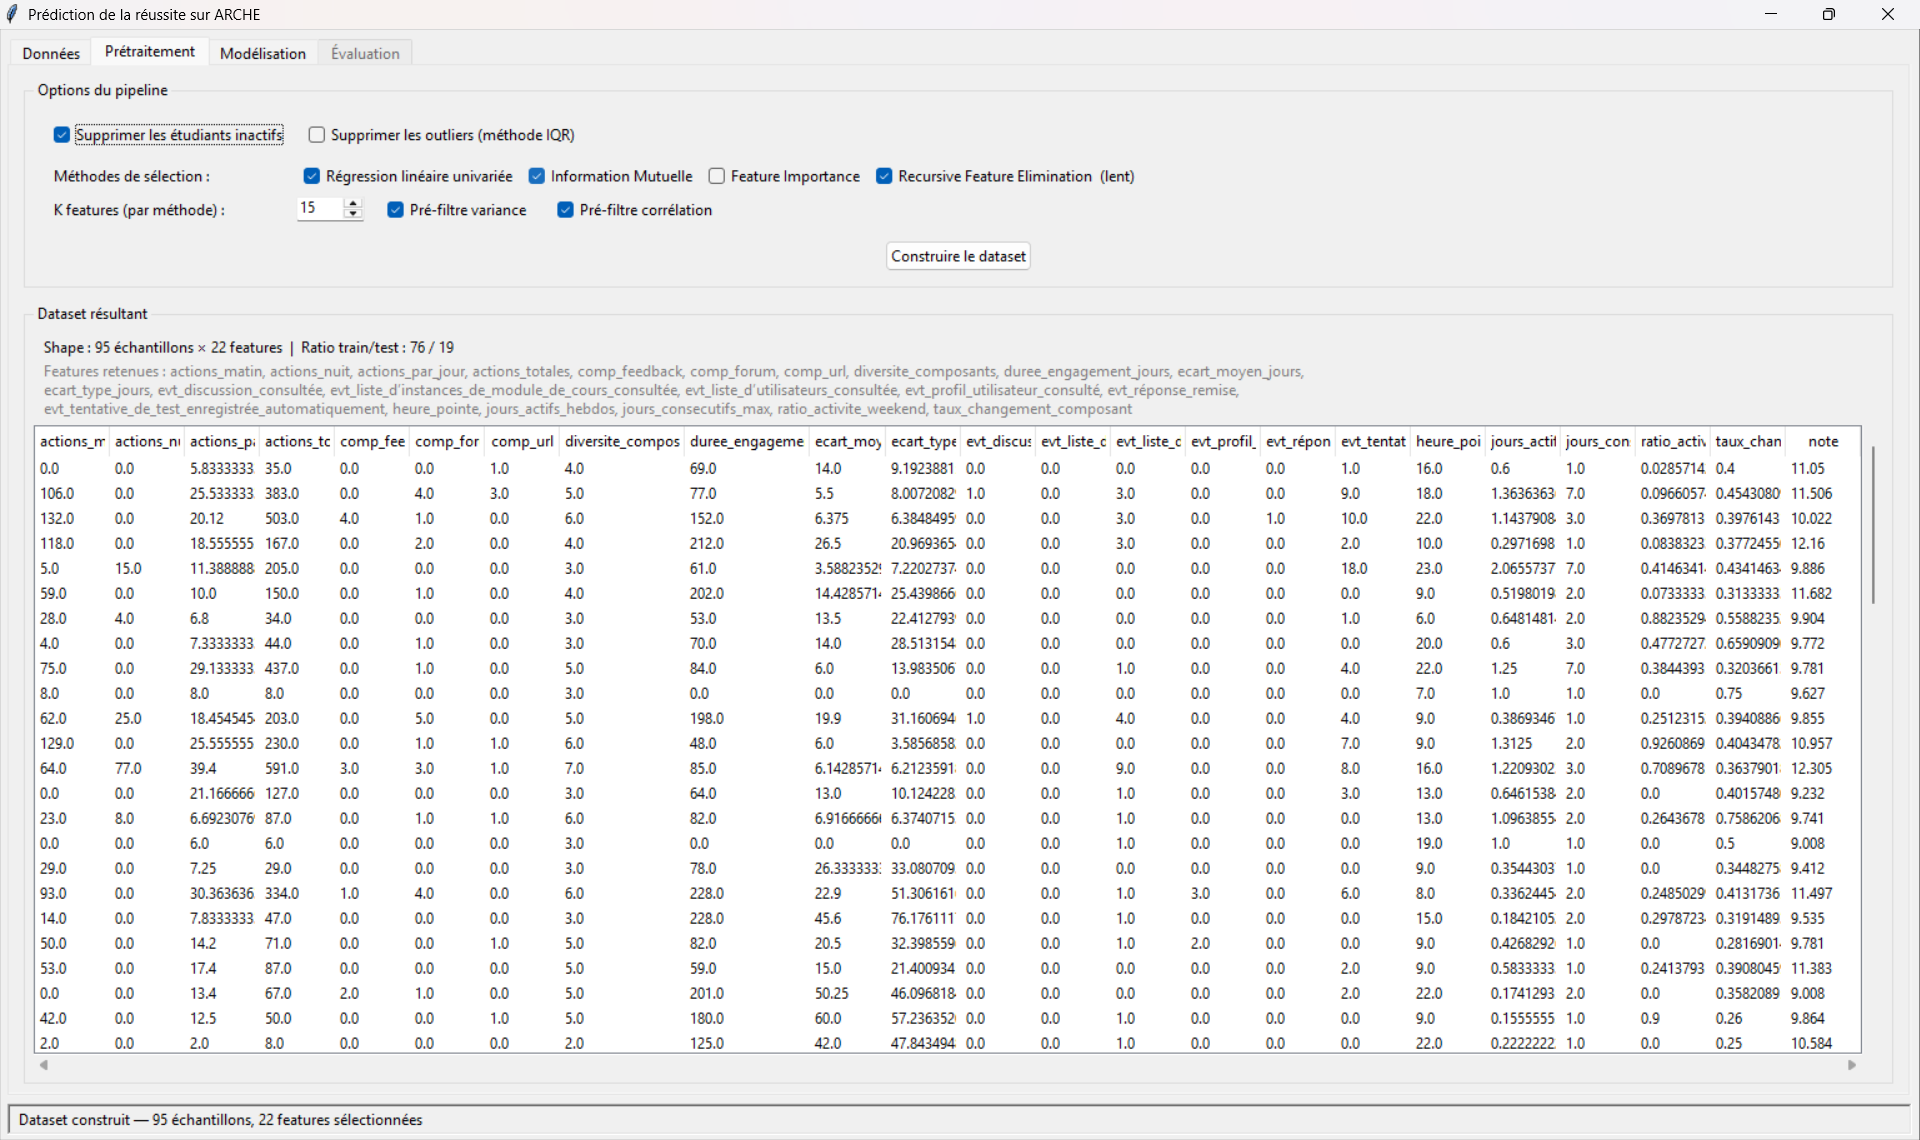
\includegraphics[width=0.92\textwidth]{../pictures/onglet2.png}
  \caption{Onglet \textit{Prétraitement} : Configuration du pipeline et dataset résultant}
\end{figure}

\noindent L'onglet \textbf{Prétraitement} expose toutes les options configurables du pipeline \texttt{DatasetBuilder} :

\begin{itemize}
  \item \textbf{Suppression des étudiants inactifs :} si coché, les étudiants présents dans les notes mais absents des logs sont exclus via un \texttt{inner join} entre les logs et les notes. Sinon, les variables manquantes sont remplacées par 0.
  \item \textbf{Suppression des outliers (IQR) :} suppression des observations statistiquement aberrantes (si la majorité des variables sont aberrantes).
  \item \textbf{Méthodes de sélection de variables :} quatre méthodes combinables (Test~F, information mutuelle, importance Random Forest, RFE).
  \item \textbf{Paramètre $k$ :} nombre de variables à retenir par méthode.
  \item \textbf{Pré-filtres :} filtre de variance quasi-nulle et filtre de colinéarité.
\end{itemize}

\section{Onglet 3 : Modélisation}

\begin{figure}[H]
  \centering
  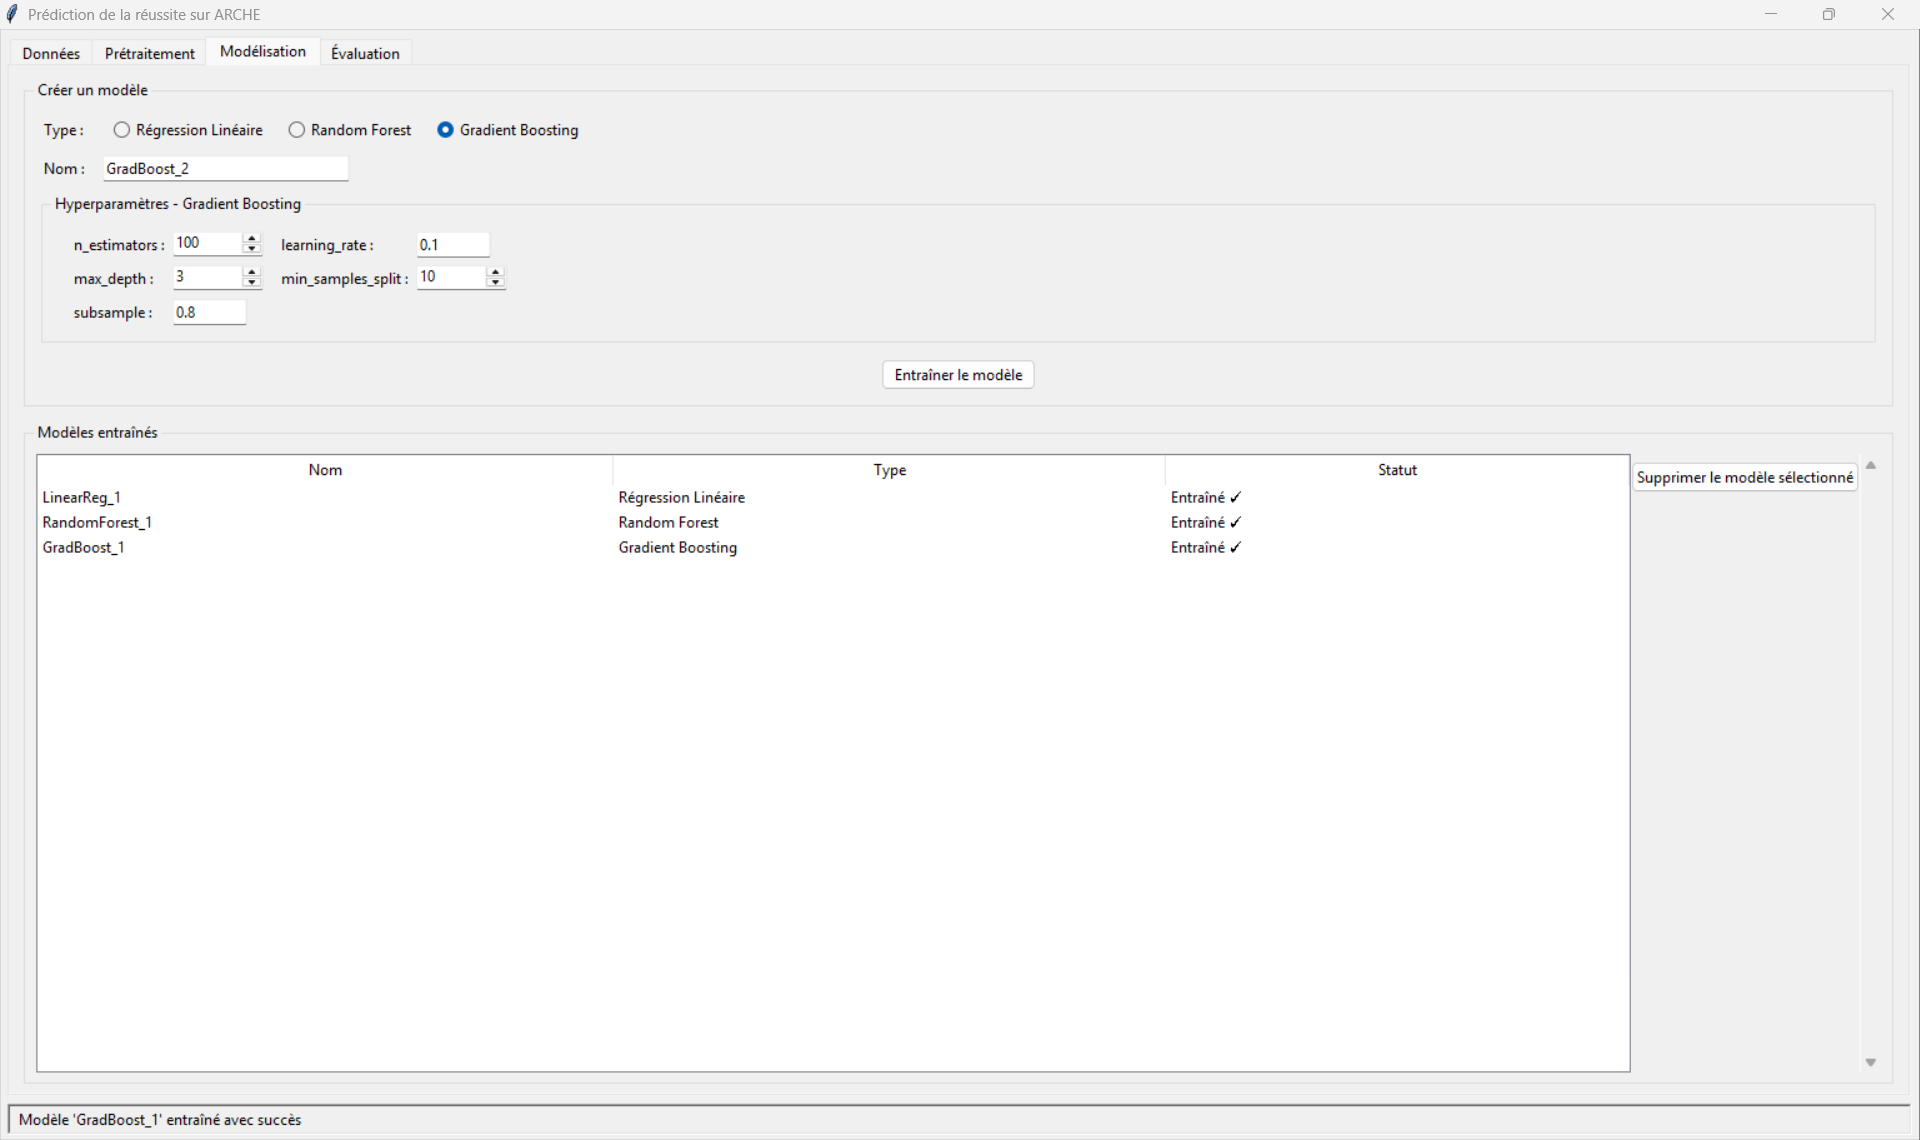
\includegraphics[width=0.92\textwidth]{../pictures/onglet3.png}
  \caption{Onglet \textit{Modélisation} -- Création et entraînement des modèles}
\end{figure}

L'onglet \textbf{Modélisation} permet de choisir le type de modèle, de le nommer, de configurer ses hyperparamètres via des spinbox dédiées, puis de lancer l'entraînement. Plusieurs modèles peuvent être entraînés simultanément pour comparaison.

\section{Onglet 4 : Évaluation}

\begin{figure}[H]
  \centering
  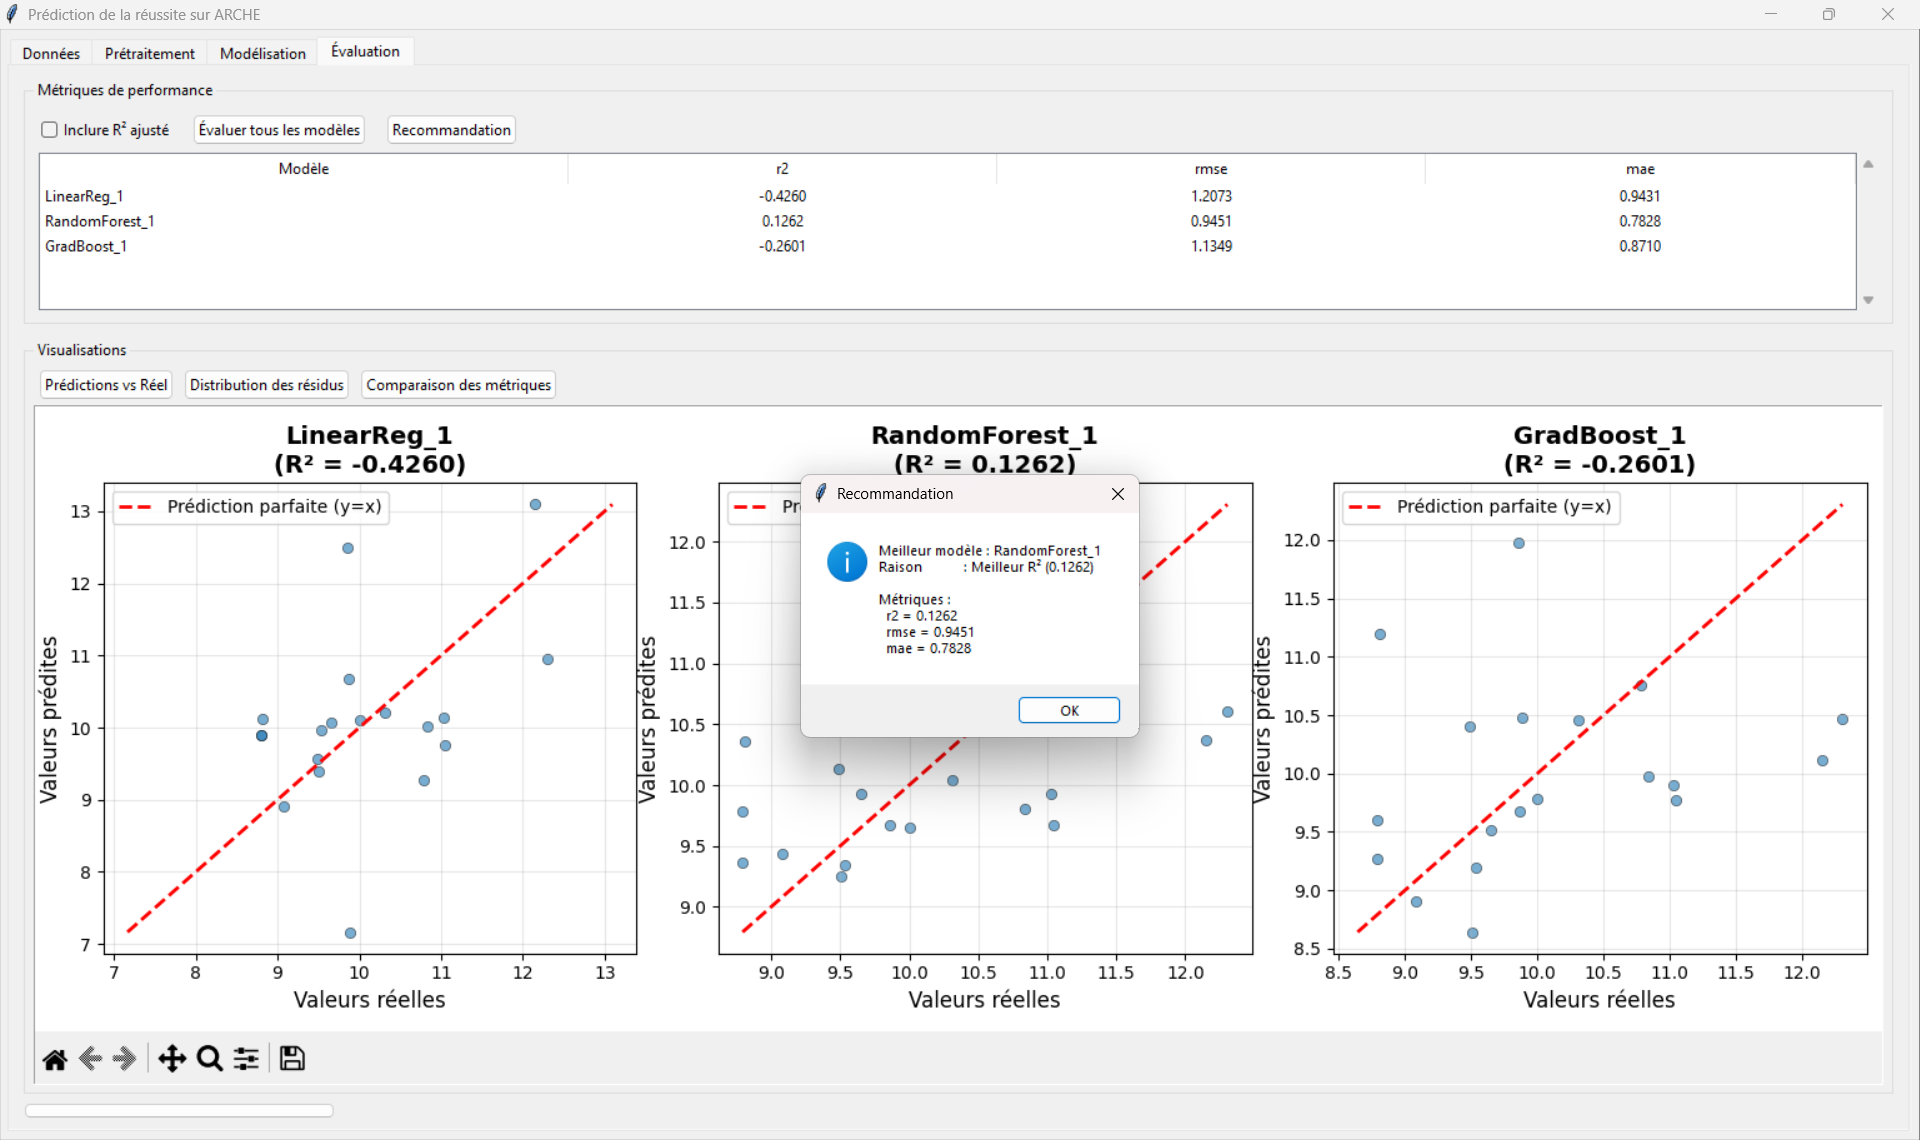
\includegraphics[width=0.92\textwidth]{../pictures/onglet4.png}
  \caption{Onglet \textit{Évaluation} -- Comparaison des modèles et visualisations}
\end{figure}

\noindent L'onglet \textbf{Évaluation} offre :
\begin{itemize}
  \item un tableau de comparaison des métriques ($R^2$, RMSE, MAE).
  \item trois sous-onglets de visualisation : prédictions vs réel, distribution des résidus, comparaison des métriques par modèle.
  \item un bouton \textit{Recommandation} analysant automatiquement les métriques.
  \item l'export de tous les résultats (CSV et images PNG) vers \texttt{output/}.
\end{itemize}

\section{Gestion asynchrone}

Toutes les opérations longues sont exécutées dans un thread secondaire afin de préserver la réactivité de l'interface Tkinter :

\begin{lstlisting}[caption={Patron de thread commun aux onglets}]
def _run_thread(self, worker, on_success, on_error=None) -> None:
    def target():
        try:
            result = worker()
            # Callback planifie dans le thread principal (Tk)
            self.frame.after(0, on_success, result)
        except Exception as exc:
            if on_error:
                self.frame.after(0, on_error, str(exc))

    threading.Thread(target=target, daemon=True).start()
\end{lstlisting}

L'utilisation de \texttt{frame.after(0, callback)} garantit que la mise à jour de l'interface se fait toujours dans le thread principal de Tkinter, conformément aux contraintes de la bibliothèque.

% ============================================================
\chapter{Principaux algorithmes}
% ============================================================

\section{Extraction de variables (Feature Engineering)}

La classe \texttt{FeatureExtractor} transforme un fichier de logs brut (une ligne par événement) en un tableau récapitulatif par étudiant.
L'extraction est découpée en cinq sous-méthodes appelées séquentiellement par \texttt{extract\_features()}.

\begin{center}
\footnotesize
\begin{tabular}{lp{7cm}r}
\toprule
\textbf{Méthode} & \textbf{Variables produites} & \textbf{Nb.}\\
\midrule
\texttt{compute\_activity\_metrics}
  & Actions totales, jours actifs, durée d'engagement, sessions & 4\\
\texttt{compute\_temporal\_patterns}
  & Heure de pointe, ratio week-end, tranches horaires, ... & 8\\
\texttt{compute\_component\_features}
  & Comptage par composant ARCHE (\texttt{comp\_*}) & variable\\
\texttt{compute\_event\_type\_features}
  & Comptage par type d'événement (\texttt{evt\_*}) & variable\\
\texttt{compute\_consistency\_features}
  & Jours consécutifs max, écarts inter-sessions, fréquence & 4\\
\texttt{compute\_interaction\_depth}
  & Actions par jour, diversité, taux de changement & 4\\
\bottomrule
\end{tabular}
\end{center}

L'algorithme pour calculer la plus longue série de jours consécutifs d'activité illustre la complexité du feature engineering :

\begin{lstlisting}[caption={Calcul du plus grand nombre de jours d'activité successif}]
def calculate_streak_days(dates):
	if len(dates) == 0:
		return 0
	if len(dates) == 1:
		return 1

	max_streak = 1
	current_streak = 1

	dates = pd.to_datetime(pd.Series(dates))
	for i in range(1, len(dates)):
		diff = (dates[i] - dates[i-1]).days
		if diff == 1:
			current_streak += 1
			max_streak = max(max_streak, current_streak)
		else:
		current_streak = 1

	return max_streak
\end{lstlisting}

\section{Sélection de variables}

La sélection des variables s'effectue en deux phases dans \texttt{DataCleaner}.

\subsection{Phase 1 : Pré-filtrage}

\begin{enumerate}
  \item \textbf{Filtre de variance quasi-nulle} (\texttt{VarianceThreshold}) : supprime les colonnes dont la variance est inférieure à 0,01, typiquement les composants ARCHE que personne n'utilise.

  \item \textbf{Filtre de colinéarité :} pour chaque paire de variables dont $|r| > 0{,}85$, la variable à plus faible variance est supprimée.
\end{enumerate}

\subsection{Phase 2 : Sélection avancée (Ensemble Feature Selection)}

Jusqu'à quatre méthodes peuvent être combinées. L'union des ensembles de variables sélectionnées par chaque méthode est retenue.

\begin{center}
\begin{tabular}{llp{5.5cm}}
\toprule
\textbf{Méthode} & \textbf{Classe sklearn} & \textbf{Principe}\\
\midrule
\texttt{linear}       & \texttt{SelectKBest(f\_regression)}           & Corrélation linéaire (Test~F)\\
\texttt{mutual\_info} & \texttt{SelectKBest(mutual\_info\_regression)} & Information mutuelle\\
\texttt{importance}   & \texttt{RandomForestRegressor}                 & Importance (Gini / MSE)\\
\texttt{rfe}          & \texttt{RFE(RandomForestRegressor)}            & Élimination récursive\\
\bottomrule
\end{tabular}
\end{center}

\section{Entraînement des modèles : Méthode Patron}

La méthode publique \texttt{fit()} de \texttt{BaseRegressor} définit
le squelette invariant de l'entraînement :

\begin{lstlisting}[caption={Template Method dans BaseRegressor}]
def fit(self, X, y) -> 'BaseRegressor':
    # 1. Validation des entrees (identique pour tous les modeles)
    self._validate_input_data(X, y)
    # 2. Standardisation (RobustScaler, identique pour tous)
    X = self.scaler.fit_transform(X)
    # 3. Entrainement specifique (implementation dans les sous-classes)
    self._fit(X, y)
    return self

@abstractmethod
def _fit(self, X, y) -> None:
    """A implementer dans chaque sous-classe."""
    pass
\end{lstlisting}

Le \texttt{RobustScaler} a été choisi car les données de logs présentent de fortes disparités (un étudiant peut avoir 10 actions, un autre plus de mille 1\,000).
Contrairement au \texttt{StandardScaler}, il utilise la médiane et l'écart interquartile, ce qui le rend robuste aux valeurs extrêmes.

\section{Métriques d'évaluation}

Trois métriques principales sont calculées pour chaque modèle :

\begin{align}
  R^2 &= 1 - \frac{\sum_i (y_i - \hat{y}_i)^2}{\sum_i (y_i - \bar{y})^2}
         \quad \in (-\infty,\, 1]\\[6pt]
  \text{RMSE} &= \sqrt{\frac{1}{n}\sum_{i=1}^{n}(y_i - \hat{y}_i)^2}\\[6pt]
  \text{MAE}  &= \frac{1}{n}\sum_{i=1}^{n}\left|y_i - \hat{y}_i\right|
\end{align}

Le \textbf{$R^2$ ajusté} est disponible en option :
\begin{equation}
  R^2_{\text{adj}} = 1 - (1-R^2)\cdot\frac{n-1}{n-p-1}
\end{equation}
où $n$ est le nombre d'observations et $p$ le nombre de variables explicatives.


% ============================================================
\chapter{Utilisation de l'intelligence artificielle générative}
% ============================================================

Dans un souci de transparence académique, ce dossier mentionne explicitement le recours à un outil d'intelligence artificielle générative, indispensable afin de pouvoir rendre ce dossier dans les délais impartis.

\section{Rôle de l'IA dans le développement}

L'assistant \textbf{Claude Code} (Anthropic, modèle Sonnet 4.6) a été utilisé tout au long du projet pour :

\begin{itemize}
  \item l'aide à la rédaction des \textit{docstrings} et de la documentation.
  \item la review de code et la rédaction des tests unitaires.
  \item génération de maquettes et plan d'actions pour l'implémentation de l'interface graphique.
  \item relecture des présents dossiers.
  \item la génération des diagrammes TikZ et UML.
\end{itemize}


\section{Limites et responsabilité}

L'ensemble du code source a été \textbf{relu, compris et validé} par l'auteur avant intégration. Les choix algorithmiques, architecturaux et d'analyse restent de la responsabilité de l'auteur.

\begin{notebox}
L'utilisation de l'IA générative est un sujet d'actualité dans l'enseignement supérieur. Considérant que la transparence est préférable à la dissimulation, et que la maîtrise des outils d'IA fait partie des compétences attendues d'un Master en Sciences des Données, ce recours est ici déclaré explicitement.
\end{notebox}

% ============================================================
% Conclusion
% ============================================================
\chapter*{Conclusion}
\addcontentsline{toc}{chapter}{Conclusion}

Ce dossier technique a présenté la conception du logiciel \textit{Projet Réussite}, développé en Python~3 en respectant les contraintes imposées (POO, sans notebook, Tkinter). L'architecture MVC assure une séparation claire des responsabilités, les patrons de conception (Template Method, Façade, Stratégie) favorisent l'extensibilité du code, et la gestion asynchrone garantit la réactivité de l'interface graphique.

L'analyse des résultats et les limites du projet sont développées dans le \textbf{Dossier d'Analyse} associé.

\end{document}
